\section{Abstract Store}
This section introduces the abstract store.
\subsection{Data Graph}
\label{graph_model}
The data structures of the virtual machine are modeled as nodes in a
directed graph with nodes and directed edges.

The data graph is built from {\em nodes}.
Each node has a type and a finite number of edges.

\begin{figure}[ht]
\centering
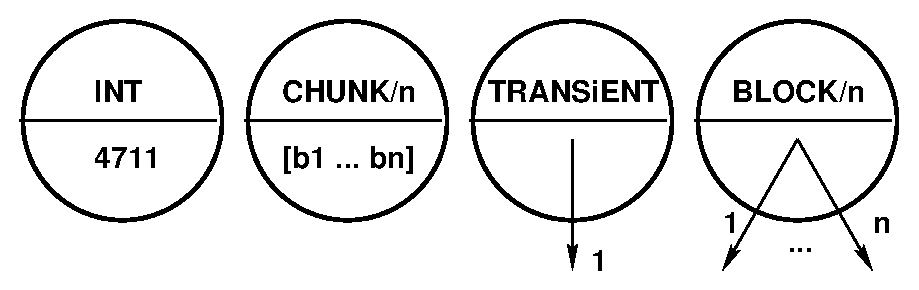
\includegraphics[width=7.0cm]{figures/graph_nodes}
\caption{\label{store_units} {\it Supported node types}}
\end{figure}

Figure \ref{store_units} shows all supported node types:
\begin{description}
\item[int]
Encapsulates integer numbers.
\item[chunk]
A chunk represents an byte array of size n. A chunk has no edges.
\item[transient]
A transient provides exactly one link which will be connected
with its value.
\item[block]
A block provides {\em n} links.
\end{description}
The data graph is built by connecting single nodes together.

A freshly created node must
have all its edges assigned before it can be connected
to a node already present in the data graph.

It is not possible to create a cycle in the graph by adding new nodes.
This requires a rewriting step.
\begin{paragraph}{Rewriting invariants.}
Exactly three graph rewriting operations are performed during computation:
\begin{description}
\item[node creation] New nodes can be created and added to the graph.
\item[binding transients] Transient nodes can be bound to other nodes.
This makes the transient tranparent in the graph. That is,
all incoming edges of the transient are redirected to the bound node.
\item[reconnecting edges] An outgoing edge of a block node can be
reconnected to a different node.
Reconnecting nodes possibly creates a cycle in the graph.
\end{description}
\end{paragraph}
\subsection{Store}
The store efficiently implements the data graph and provides for
automatic garbage collection.

The store provides the following operations on nodes:
\begin{itemize}
\item Creating single nodes
\item Connecting nodes to a graph
\item Reconnecting nodes to a graph
\item Accessing values within the graph
\end{itemize}
The store distinguishes first time connection
and reconnecting a previously assigned edge. This is a consequence
of the underlying generational gc which requires a write barrier in general.

Accessing values in the data graph requires the interleaved iteration of
\begin{enumerate}
\item decoding the node's value
\item accessing the $i$-th edge
\end{enumerate}
\begin{paragraph}{Decoding values.}
The decode operation on nodes is a type case which delivers
the encoded value. The type case makes bound transients transparent
in the graph as described in section \ref{graph_model}.
\end{paragraph}
\begin{paragraph}{Accessing edges.}
Each block provides a read, init and write accessor to its edges.
Each access is performed with a bounds check to ensure data integrity.
\end{paragraph}
\begin{paragraph}{Refined value access.}
The value access as described above is safe for all store data structures
but involves some overhead. This is due to the type tests and the
dereferencing of bound transients.

The store provides a second interface level which requires the user
to know what types he operates on. This interface decodes values directly
without error checking and does not respect the transient semantics.

This allows for both expressing invariants
and greater performance in the resulting code.

This interface is used to built the abstract datatypes already provided
with the system.
\end{paragraph}
